\par Complementary metal oxide semiconductor (CMOS) sensors are one of the most common modern methods of creating digital image sensors. \autoref{fig:filters} illustrates how light passing from the outside passes through a glass lens and a color filter before finally reaching the photo-diodes.
\begin{figure}[H]
    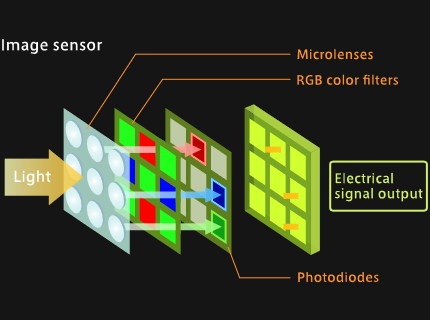
\includegraphics[width=\linewidth]{ImageSensor}
    \caption{CMOS Image Sensor\cite{Tokyo_Electron_Committee}}
    \label{fig:filters}
\end{figure}
\par The photo-diode is sensitive to light and is able to generate a current when exposed to photons. Lastly, that signal is sent to a central processor and translated into a pixel\cite{Tokyo_Electron_Committee}. Because of the required exposure to photons, CMOS sensors receive excessive radiation emissions and are vulnerable to a higher than noraml number of faults. \autoref{fig:CMOS} shows a basic schematic for a CMOS sensor. The photo diode has to be exposed to the incoming light so that it can activate the circuit, however, this makes it vulnerable to any other interference that can potentially harm the sensor. 
\begin{figure}[H]
    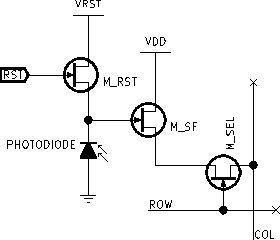
\includegraphics[width=\linewidth]{cmosSch}
    \caption{Three Transistor Active Pixel}
    \label{fig:CMOS}
\end{figure}
\par One fault that often occurs in CMOS sensors is dark current. A dark current is when the CMOS circuit is activated by a wave that is not a photon \cite{mcgrath_tobin_goiffon_magan_2018}. In radiation intensive environments this is a relevant limitation of the technology because extreme accuracy is required with very high consistency. Radiation that reaches a sensor is likely to cause some kind of fault, and if the intensity of the radiation is high enough a pixel can become permanently damaged \cite{bardoux_penquer_gilard_ecoffet_auvergne_2017}. These Dark Currents when realized through the circuit and the central processor would appear to be noise or a collection of white pixels. These faults can be harmless to the sensor at first, but given enough time to build up they can render a sensor useless. 